\documentclass[12pt]{article}
\usepackage{amsmath}
\usepackage{graphicx}
\usepackage{hyperref}
\usepackage{listings}
\usepackage{color}
\usepackage{pythonhighlight}

\title{Operating System Course Report - First Half of the Semester}
\author{A class}
\date{\today}

\begin{document}

\maketitle
\newpage

\tableofcontents
\newpage

\section{Introduction}
This report summarizes the topics covered during the first half of the Operating System course. It includes theoretical concepts, practical implementations, and assignments. The course focuses on the fundamentals of operating systems, including system architecture, process management, CPU scheduling, and deadlock handling.

\section{Course Overview}
\subsection{Objectives}
The main objectives of this course are:
\begin{itemize}
    \item To understand the basic components and architecture of a computer system.
    \item To learn process management, scheduling, and inter-process communication.
    \item To explore file systems, input/output management, and virtualization.
    \item To study the prevention and handling of deadlocks in operating systems.
\end{itemize}

\subsection{Course Structure}
The course is divided into two halves. This report focuses on the first half, which covers:
\begin{itemize}
    \item Basic Concepts and Components of Computer Systems
    \item System Performance and Metrics
    \item System Architecture of Computer Systems
    \item Process Description and Control
    \item Scheduling Algorithms
    \item Process Creation and Termination
    \item Introduction to Threads
    \item File Systems
    \item Input and Output Management
    \item Deadlock Introduction and Prevention
    \item User Interface Management
    \item Virtualization in Operating Systems
\end{itemize}

\section{Topics Covered}

\subsection{Basic Concepts and Components of Computer Systems}
This section explains the fundamental components that make up a computer system, including the CPU, memory, storage, and input/output devices.

\subsection{System Performance and Metrics}
This section introduces various system performance metrics used to measure the efficiency of a computer system, including throughput, response time, and utilization.

\subsection{System Architecture of Computer Systems}
Describes the architecture of modern computer systems, focusing on the interaction between hardware and the operating system.

\subsection{Process Description and Control}
Processes are a central concept in operating systems. This section covers:
\begin{itemize}
    \item Process states and state transitions
    \item Process control block (PCB)
    \item Context switching
\end{itemize}

\subsection{Scheduling Algorithms}
This section covers:
\begin{itemize}
    \item First-Come, First-Served (FCFS)
    \item Shortest Job Next (SJN)
    \item Round Robin (RR)
\end{itemize}
It explains how these algorithms are used to allocate CPU time to processes.

\subsection{Process Creation and Termination}
Details how processes are created and terminated by the operating system, including:
\begin{itemize}
    \item Process spawning
    \item Process termination conditions
\end{itemize}

\subsection{Introduction to Threads}
This section introduces the concept of threads and their relation to processes, covering:
\begin{itemize}
    \item Single-threaded vs. multi-threaded processes
    \item Benefits of multithreading
\end{itemize}

\begin{figure}[h]
    \centering
    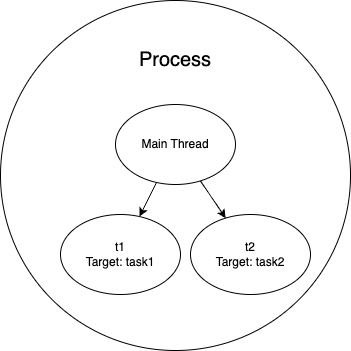
\includegraphics[width=0.5\textwidth]{/Users/khawaritzmi/Unhas/os_report_mid2024/a_class/asset/example.png}  % Sesuaikan nama file dan ukurannya
    \caption{Ini adalah gambar contoh dari multithreading.}
    \label{fig:contoh_gambar}
\end{figure}

Seperti yang terlihat pada Gambar \ref{fig:contoh_gambar}, inilah cara menambahkan gambar dengan keterangan.

\subsection{File Systems}
File systems provide a way for the operating system to store, retrieve, and manage data. This section explains:
\begin{itemize}
    \item File system structure
    \item File access methods
    \item Directory management
\end{itemize}

\subsection{Input and Output Management}
Input and output management is key for handling the interaction between the system and external devices. This section includes:
\begin{itemize}
    \item Device drivers
    \item I/O scheduling
\end{itemize}

\subsection{Deadlock Introduction and Prevention}
Explores the concept of deadlocks and methods for preventing them:
\begin{itemize}
    \item Deadlock conditions
    \item Deadlock prevention techniques
\end{itemize}

\subsection{User Interface Management}


 adalah proses merancang, mengimplementasi, dan memelihara unsur-unsur interaktif dari sebuah sistem perangkat lunak yang memungkinkan pengguna untuk berinteraksi dengan fungsi sistem tersebut.

  Shneiderman(2016) Menjelaskan tentang proses merancang dari sebuah sistem 
 

\subsubsection{Jenis-Jenis User Interface}
\par Antarmuka pengguna (\textit{User Interface}) dapat didefinisikan sebagai bagian dari sistem komputer yang memungkinkan manusia berinteraksi dengan dan melakukan tugas-tugas pada sistem komputer tersebut. Perkembangan antarmuka pengguna telah menghasilkan beberapa jenis utama. 



\begin{enumerate}
    \item{\textit{Graphical User Interfaces} (GUI)

 adalah jenis antarmuka yang digunakan oleh pengguna untuk berinteraksi dengan sistem operasi melalui gambar-gambar grafis, ikon, menu, dan menggunakan alat penunjuk (\textit{pointing device}) seperti tetikus atau bola jejak. Unsur-unsur utama dari GUI bisa diringkas dalam konsep JIMA (\textit{jendela, ikon, menu, alat penunjuk})

 Shneiderman(2016) Menjelaskan tugas tugas komputer yang memungkinkan pengguna  berinteraksi dengan sistem operasi


 \item\textit{Command Line Interface} (CLI)

 adalah jenis antarmuka di mana pengguna berinteraksi dengan sistem operasi melalui terminal teks. Pengguna menjalankan perintah dan program di sistem operasi tersebut dengan cara mengetikkan baris-baris tertentu.

 Shneiderman(2016) Menjelaskan pengguna berinteraksi dengan sistem operasi. 


\item{\textit{Text User Interface} (TUI)}

 merupakan bentuk antarmuka yang menggabungkan unsur CLI dan GUI. Antarmuka ini menggunakan karakter teks untuk menciptakan tampilan semi-grafis. TUI menawarkan navigasi yang lebih mudah dibandingkan CLI, namun tetap mempertahankan efisiensi penggunaan sumber daya sistem yang rendah. TUI sering digunakan pada sistem operasi berbasis teks atau aplikasi yang memerlukan tampilan sederhana namun fungsional.

McTear (2016) menjelaskan betuk antarmuka yang menggabungkan unsur CLI  dan GUI 

\item {\textit{Voice User Interface} (VUI)}

 adalah jenis antarmuka yang memungkinkan pengguna berinteraksi dengan sistem menggunakan suara. Teknologi ini memanfaatkan pemrosesan bahasa alami dan pengenalan suara untuk menerjemahkan perintah lisan menjadi tindakan yang dapat dijalankan oleh sistem. VUI telah menjadi semakin populer dengan munculnya asisten virtual seperti Siri, Alexa, dan Google Assistant.

McTear (2016) menjelaskan pengguna berinteraksi dengan sistem menggunakan suara

\item{\textit{Conversational User Interface} (CUI)}

 merupakan pengembangan lebih lanjut dari VUI, yang memungkinkan interaksi yang lebih alami dan kontekstual antara pengguna dan sistem. CUI tidak hanya mengandalkan perintah suara, tetapi juga dapat menggunakan teks, seperti yang terlihat pada robot obrolan dan\textit{ asisten virtual }berbasis teks. CUI dirancang untuk memahami konteks percakapan dan memberikan tanggapan yang lebih personal dan relevan.
 
 McTear (2016) menjelaskan betuk antarmuka yang menggabungkan unsur CLI  dan GUI

\end{enumerate}

\subsubsection{Interaksi antara Pengguna dan Sistem Operasi}

Interaksi antara pengguna dan sistem operasi adalah proses komunikasi dua arah yang memungkinkan pengguna untuk mengendalikan dan menggunakan fungsi-fungsi komputer melalui berbagai jenis antarmuka. Aspek-aspek kunci dalam interaksi pengguna-sistem operasi:

Raymond(2003) menjelaskan tentang interaksi antara dan sistem operasi

\begin{enumerate}
\item \textit{Graphical User Interfaces } (GUI) menjadi pilihan utama bagi kebanyakan pengguna karena kemudahannya. Melalui GUI, pengguna dapat mengelola berkas, folder, dan aplikasi dengan mudah menggunakan tetikus atau layar sentuh. Ikon, jendela, dan menu yang disediakan memungkinkan navigasi yang intuitif dalam sistem berkas dan pengoperasian berbagai fungsi komputer. Di sisi lain, \item{Command Line Interface (CLI)} tetap menjadi pilihan bagi pengguna tingkat lanjut dan administrator sistem. CLI menawarkan kendali yang lebih tepat dan kemampuan untuk mengotomatisasi tugas-tugas kompleks melalui skrip.

\item {Manajemen Berkas dan Direktori} menjadi lebih mudah dengan adanya representasi visual dalam GUI, sementara CLI menyediakan perintah-perintah yang memungkinkan manipulasi berkas secara efisien. Pengguna dapat dengan mudah membuat, menghapus, memindahkan, dan mengatur berkas serta folder sesuai kebutuhan mereka.

\item {Manajemen Proses} sistem operasi memungkinkan pengguna untuk memulai, menghentikan, dan memantau\textit{ aplikasi} yang berjalan. GUI menyediakan \textit{pengelola tugas} yang memvisualisasikan proses yang sedang berjalan, sementara CLI menawarkan perintah-perintah untuk mengelola proses dengan tingkat kendali yang lebih tinggi.

\item {Konfigurasi Sistem} menjadi lebih mudah diakses melalui panel kendali atau pengaturan dalam GUI, memungkinkan pengguna untuk menyesuaikan berbagai aspek sistem operasi. Sementara itu memungkinkan konfigurasi yang lebih mendalam melalui berkas konfigurasi dan perintah-perintah khusus.

\item {Keamanan dan otentikasi} merupakan aspek penting dalam interaksi pengguna-sistem. Sistem operasi menyediakan mekanisme masuk dan manajemen hak akses untuk melindungi data dan sumber daya sistem. GUI menawarkan dialog visual yang ramah pengguna untuk proses otentikasi, sementara CLI menggunakan \textit{prompt} teks yang sederhana namun aman.

\item {Pembaruan dan pemeliharaan sistem} menjadi lebih mudah dengan adanya pemberitahuan visual dan panduan dalam GUI. Sementara itu, CLI memungkinkan administrator sistem untuk melakukan pembaruan dan pemeliharaan melalui perintah dan skrip yang dapat diotomatisasi.

\item{Aksesibilitas} menjadi fokus penting dalam pengembangan antarmuka modern. Antarmuka Pengguna Suara (VUI) dan Antarmuka Pengguna Percakapan (CUI) meningkatkan aksesibilitas bagi pengguna dengan kebutuhan khusus. Fitur seperti pembaca layar dan kendali suara terintegrasi dengan baik dalam sistem operasi modern, memastikan bahwa teknologi dapat diakses oleh semua kalangan.

Cohen(2004) Menjelaskan tentang pentingnya fokus dalam pengembangan antarmuka 
\end{enumerate}

\begin{thebibliography}{9} 

\bibitem{Shneiderman2016}
Shneiderman, B., Plaisant, C., Cohen, M., Jacobs, S., Elmqvist, N., \& Diakopoulos, N. (2016). \textit{Designing the User Interface: Strategies for Effective Human-Computer Interaction} (6th ed.). Pearson.

\bibitem{McTear2016}
McTear, M., Callejas, Z., \& Griol, D. (2016). \textit{The conversational interface: Talking to smart devices}. Springer.

\bibitem{Raymond2003}
Raymond, E. S. (2003). \textit{The art of Unix programming}. Addison--Wesley Professional. 

\bibitem{Cohen2004}
Cohen, M. H., Giangola, J. P., \& Balogh, J. (2004). \textit{Voice user interface design}. Addison--Wesley Professional.

\bibitem{Reynaldi2019}
Reynaldi, A. (2019). \textit{Perancangan desain antarmuka pengguna (UI) aplikasi pencari kos} [Skripsi tidak diterbitkan]. Program Studi Desain Komunikasi Visual, Fakultas Seni dan Desain, Universitas Negeri Makassar


			

\end{thebibliography}




\subsection{Virtualization in Operating Systems}
Virtualization allows multiple operating systems to run concurrently on a single physical machine. This section explores:
\begin{itemize}
    \item Concept of virtualization
    \item Hypervisors and their types
    \item Benefits of virtualization in modern computing
\end{itemize}

\section{Assignments and Practical Work}
\subsection{Assignment 1: Process Scheduling}
Students were tasked with implementing various process scheduling algorithms (e.g., FCFS, SJN, and RR) and comparing their performance under different conditions.
\subsubsection{Group 1}
\begin{python}
    class Process:
    def __init__(self, pid, arrival_time, burst_time):
        self.pid = pid
        self.arrival_time = arrival_time
        self.burst_time = burst_time
        self.completion_time = 0
        self.turnaround_time = 0
        self.waiting_time = 0
\end{python}

\subsubsection{Kelompok 12}

\definecolor{codegreen}{rgb}{0,0.6,0}
\definecolor{codegray}{rgb}{0.5,0.5,0.5}
\definecolor{codepurple}{rgb}{0.58,0,0.82}
\definecolor{backcolour}{rgb}{0.95,0.95,0.92}

\lstdefinestyle{mystyle}{
    backgroundcolor=\color{backcolour},   
    commentstyle=\color{codegreen},
    keywordstyle=\color{magenta},
    numberstyle=\tiny\color{codegray},
    stringstyle=\color{codepurple},
    basicstyle=\ttfamily\footnotesize,
    breakatwhitespace=false,         
    breaklines=true,                 
    captionpos=b,                    
    keepspaces=true,                 
    numbers=left,                    
    numbersep=5pt,                  
    showspaces=false,                
    showstringspaces=false,
    showtabs=false,                  
    tabsize=2
}

\lstset{style=mystyle}


\begin{tabular}{|c|c|c|}
  \hline
  \textbf{Proses} & \textbf{Waktu Kedatangan} & \textbf{Waktu Burst} \\
  \hline
  P1 & 0 & 10 \\
  \hline
  P2 & 1 & 6 \\
  \hline
  P3 & 3 & 2 \\
  \hline
  P4 & 5 & 4 \\
  \hline
  P5 & 6 & 8 \\
  \hline
\end{tabular}


\paragraph{Pertanyaan:} Buatlah jadwal eksekusi kelima proses tersebut menggunakan algoritma FCFS Hitunglah:
   \begin{itemize}
      \item[a.] Waktu penyelesaian (Completion Time) setiap proses
      \item[b.] Waktu turnaround (Turnaround Time) setiap proses
      \item[c.] Waktu tunggu (Waiting Time) setiap proses
      \item[d.] Rata-rata waktu turnaround
      \item[e.] Rata-rata waktu tunggu
   \end{itemize}

Serta berikan juga diagram Gantt untuk masing-masing algoritma untuk memvisualisasikan urutan eksekusi prosesnya.

\paragraph{Jawaban:} 

First-Come, First-Served (FCFS) Algorithm

\begin{lstlisting}[]
def fcfs(processes):
    time = 0
    result = []
    gantt = []
    for process in sorted(processes, key=lambda p: p.arrival_time):
        if time < process.arrival_time:
            time = process.arrival_time
        process.completion_time = time + process.burst_time
        process.turnaround_time = process.completion_time - process.arrival_time
        process.waiting_time = process.turnaround_time - process.burst_time
        gantt.extend([process.pid] * process.burst_time)
        time = process.completion_time
        result.append(copy.deepcopy(process))
    return result, gantt
\end{lstlisting}



\section*{Output Code:}

Process 1: CT=10, TAT=10, WT=0 \\
Process 2: CT=16, TAT=15, WT=9 \\
Process 3: CT=18, TAT=15, WT=13 \\
Process 4: CT=22, TAT=17, WT=13 \\
Process 5: CT=30, TAT=24, WT=16 \\

Average Turnaround Time: 16.20 \\
Average Waiting Time: 10.20

\subsection*{Gantt Chart}

\begin{verbatim}
| P1 | P1 | P1 | P1 | P1 | P1 | P1 | P1 | P1 | P1 | P2 | P2 | P2 | P2 | P2 | P2 | P3 | P3 | P4 | P4 | P4 | P4 | P5 | P5 | P5 | P5 | P5 | P5 | P5 | P5 |
0 1 2 3 4 5 6 7 8 9 10 11 12 13 14 15 16 17 18 19 20 21 22 23 24 25 26 27 28 29 30
\end{verbatim}




\subsection{Assignment 2: Deadlock Handling}
In this assignment, students were asked to simulate different deadlock scenarios and explore various prevention methods.


\subsubsection{Group 12}

\paragraph{Pertanyaan:} Jelaskan perbedaan antara metode pencegahan dan metode penanganan deadlock!

\paragraph{Jawaban:} 
\begin{itemize}
    \item Pencegahan Deadlock: Metode ini berusaha mencegah deadlock dengan memastikan bahwa setidaknya satu dari empat kondisi deadlock tidak pernah terjadi. Misalnya, dengan menggunakan alokasi sumber daya secara hati-hati sehingga tidak ada proses yang dapat menahan dan menunggu sumber daya lainnya (melanggar kondisi "hold and wait").

    \item Penanganan Deadlock: Metode ini membiarkan deadlock terjadi, kemudian mendeteksinya, dan mengambil langkah-langkah untuk menyelesaikan situasi tersebut. Misalnya, dengan membatalkan salah satu atau beberapa proses untuk memutus siklus deadlock.
\end{itemize}



\subsection{Assignment 3: Multithreading and Amdahl's Law}
This assignment involved designing a multithreading scenario to solve a computationally intensive problem. Students then applied **Amdahl's Law** to calculate the theoretical speedup of the program as the number of threads increased.
\subsubsection{Kelompok 12}
\paragraph{Pertanyaan:} Mengapa speedup dari program paralel tidak terus meningkat secara linear seiring dengan peningkatan jumlah thread? Jelaskan berdasarkan Amdahl's Law.

\paragraph{Jawaban:} Berdasarkan Amdahl's Law, peningkatan jumlah thread tidak menghasilkan peningkatan speedup secara linear karena selalu ada bagian dari program yang tidak dapat diparalelkan (bagian serial). Meskipun jumlah thread ditingkatkan, bagian serial tersebut tetap menjadi penghambat sehingga membatasi peningkatan speedup secara keseluruhan. Saat jumlah thread meningkat, kontribusi bagian serial semakin dominan, sehingga limitasi ini menyebabkan speedup mendekati nilai maksimum tertentu, tetapi tidak terus meningkat secara linear.

Berdasarkan Amdahl's Law, peningkatan jumlah thread tidak menghasilkan peningkatan speedup secara linear karena selalu ada bagian dari program yang tidak dapat diparalelkan (bagian serial). Meskipun jumlah thread ditingkatkan, bagian serial tersebut tetap menjadi penghambat sehingga membatasi peningkatan speedup secara keseluruhan. Saat jumlah thread meningkat, kontribusi bagian serial semakin dominan, sehingga limitasi ini menyebabkan speedup mendekati nilai maksimum tertentu, tetapi tidak terus meningkat secara linear.


\subsection{Assignment 4: Simple Command-Line Interface (CLI) for User Interface Management}
Students were tasked with creating a simple **CLI** for user interface management. The CLI should support basic commands such as file manipulation (creating, listing, and deleting files), process management, and system status reporting.


\definecolor{codebg}{rgb}{0.95,0.95,0.92}  
\definecolor{keywordcolor}{rgb}{0.31,0.56,0.71}  
\definecolor{commentcolor}{rgb}{0.4,0.6,0.4} 
\definecolor{stringcolor}{rgb}{0.71,0.45,0.32}  
\definecolor{framecolor}{rgb}{0.65,0.65,0.65}  

\lstset{
    backgroundcolor=\color{codebg},   
    basicstyle=\ttfamily\small,  
    keywordstyle=\color{keywordcolor}\bfseries,
    commentstyle=\color{commentcolor}\itshape,
    stringstyle=\color{stringcolor},
    showstringspaces=false,
    frame=single,
    framesep=8pt,
    framerule=0.8pt,
    rulecolor=\color{framecolor},
    breaklines=true,  
    linewidth=\textwidth, 
    xleftmargin=0.5cm, 
    xrightmargin=0.5cm, 
    escapeinside={(*@}{@*)},  
    language=Python  
}

\subsubsection{Kelompok 12}

\paragraph{Pertanyaan:}
Ali adalah seorang programmer yang baru belajar membuat program untuk mengelola file di komputer menggunakan Command-Line Interface (CLI). Suatu hari, Ali diminta oleh gurunya untuk membuat program yang bisa:

\begin{enumerate}
    \item[a.] Membuat file baru dengan nama dan isi yang diberikan pengguna.
    \item[b.] Menampilkan daftar file yang ada di folder tempat program dijalankan.
    \item[c.] Menghapus file berdasarkan nama yang diberikan pengguna.
\end{enumerate}

Ali mencoba menulis program tersebut menggunakan bahasa Python, tapi dia bingung bagaimana cara menggabungkan ketiga fungsi tersebut ke dalam satu program. Bantu Ali untuk menyelesaikan masalah ini dengan memberikan contoh kode Python yang dapat menjalankan ketiga fungsi di atas!


\paragraph{Jawaban:}

\begin{lstlisting}[language=Python]
import os  

def create_file():
    filename = input("Masukkan nama file: ")
    content = input("Masukkan isi file: ")
    with open(filename, 'w') as file:
        file.write(content)
    print(f"File '{filename}' berhasil dibuat.\n")

def list_files():
    print("Daftar file di direktori saat ini:")
    files = os.listdir('.')  
    for file in files:
        if os.path.isfile(file):  
            print(f"- {file}")
    print()

def delete_file():
    filename = input("Masukkan nama file yang ingin dihapus: ")
    if os.path.exists(filename): 
        os.remove(filename)
        print(f"File '{filename}' berhasil dihapus.\n")
    else:
        print(f"File '{filename}' tidak ditemukan.\n")

def main():
    while True:
        print("=== Menu CLI ===")
        print("1. Buat file baru")
        print("2. Lihat daftar file")
        print("3. Hapus file")
        print("4. Keluar")
        choice = input("Pilih opsi (1/2/3/4): ")
        if choice == '1':
            create_file()
        elif choice == '2':
            list_files()
        elif choice == '3':
            delete_file()
        elif choice == '4':
            print("Program selesai.")
            break
        else:
            print("Pilihan tidak valid, coba lagi.\n")

if __name__ == "__main__":
    main()
\end{lstlisting}


\textbf{Contoh Keluaran}:


\begin{figure}[h]
    \centering
    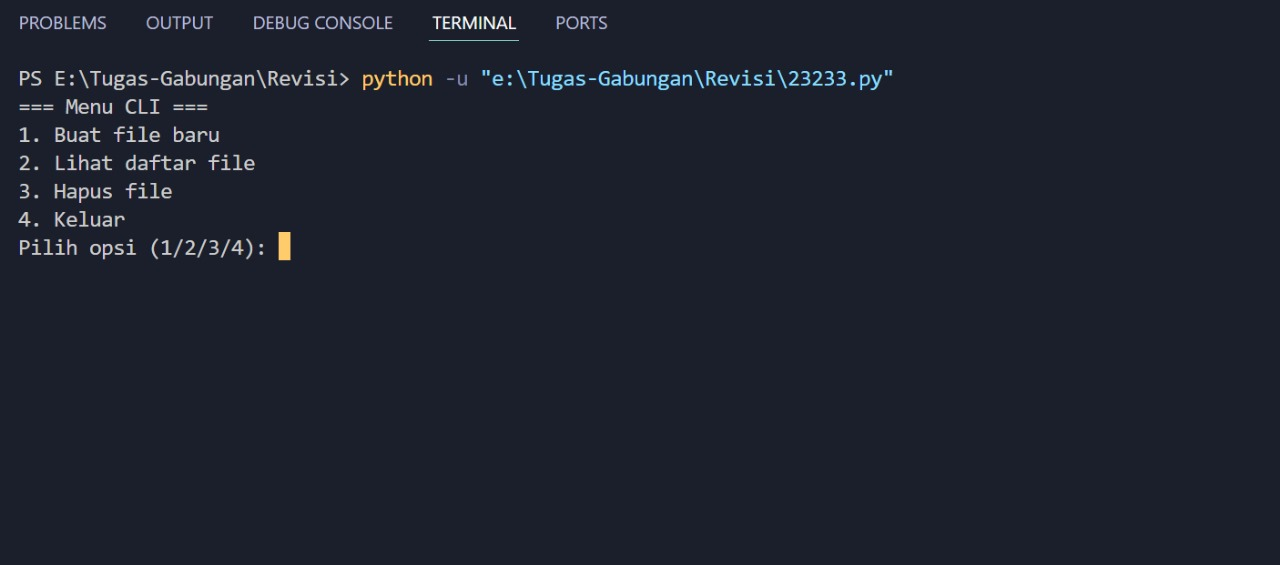
\includegraphics[width=0.5\textwidth]{asset/Output_Asignment4.jpg}
    \label{fig:contohgambar}
\end{figure}



\subsection{Assignment 5: File System Access}
In this assignment, students implemented file system access routines, including:
\begin{itemize}
    \item File creation and deletion
    \item Reading from and writing to files
    \item Navigating directories and managing file permissions
\end{itemize}

\subsubsection{Kelompok 12}b

\paragraph{Pertanyaan:} Bagaimana mekanisme pengaturan izin akses langsung ke sistem berkas lokal dari aplikasi web melalui \textit{API File System Access }dalam konteks keamanan data, dan bagaimana cara pengembang dapat memastikan bahwa izin yang diberikan kepada aplikasi hanya terbatas pada direktori yang spesifik tanpa menimbulkan potensi risiko pengungkapan data di luar cakupan yang dimaksud?

\paragraph{Jawaban:} Mekanisme pengaturan izin akses dalam File System Access API memungkinkan aplikasi web untuk berinteraksi langsung dengan sistem berkas lokal pengguna. Akses ini dilakukan berdasarkan izin yang diberikan pengguna secara eksplisit, sehingga pengembang harus memastikan aplikasi hanya meminta izin untuk berkas atau direktori yang diperlukan.

Untuk meningkatkan keamanan, penting untuk menerapkan scoped access permissions agar aplikasi tidak dapat mengakses berkas di luar cakupan izin. Pengembang juga perlu waspada terhadap potensi serangan seperti directory traversal attacks dengan melakukan path sanitization. Penggunaan persisted permissions harus dikelola dengan hati-hati agar tidak mengorbankan privasi pengguna. Dengan langkah-langkah ini, aplikasi dapat berfungsi efektif tanpa risiko mengungkapkan data sensitif.



\section{Conclusion}
The first half of the course introduced core operating system concepts, including process management, scheduling, multithreading, and file system access. These topics provided a foundation for more advanced topics to be covered in the second half of the course.

\end{document}